\documentclass[11pt]{article}
\usepackage[margin=1in]{geometry}
\usepackage{fontspec}
\usepackage{amsmath,amssymb,amsthm}
\usepackage{booktabs,array,float,graphicx}
\usepackage[font=small,labelfont=bf]{caption}
\usepackage{natbib,xurl}
\usepackage[hidelinks]{hyperref}
\usepackage{setspace}
\setstretch{1.15}
\graphicspath{{../figs/}}
% Generated by the analysis pipeline; do not edit.
\newcommand{\idMcN}{557}
\newcommand{\idScaleN}{502}
\newcommand{\idMcPositive}{125}
\newcommand{\idScalePositive}{30}
\newcommand{\idMcMissing}{0}
\newcommand{\idScaleMissing}{0}
\newcommand{\idMcRate}{22.4\%}
\newcommand{\idScaleRate}{6.0\%}
\newcommand{\idLowPrevalence}{3.0\%}
\newcommand{\idHighPrevalence}{61.2\%}
\newcommand{\idTenBounds}{$\varnothing$}
\newcommand{\idTenOuter}{[9.5, 9.8]}
\newcommand{\idTwentyBounds}{[3.1, 7.5]}
\newcommand{\idTwentyOuter}{[0.0, 11.0]}
\newcommand{\idJointComplete}{502}
\newcommand{\idJointExcluded}{0}
\newcommand{\idBothEndpoints}{4.8\%}

\newcommand{\TableStyle}{\small\setlength{\tabcolsep}{6pt}\renewcommand{\arraystretch}{1}}
\newcommand{\BeliefTableStyle}{\footnotesize\setlength{\tabcolsep}{2pt}\renewcommand{\arraystretch}{1}}
\newcommand{\PropositionTableStyle}{\footnotesize\setlength{\tabcolsep}{3pt}\renewcommand{\arraystretch}{1}}

\newtheorem{proposition}{Proposition}
\newcommand{\states}{\mathcal{S}}
\newcommand{\simplex}{\Delta^4}

\title{The Waters of Casablanca: On Political Misinformation}
\author{Robert C. Luskin \and Gaurav Sood}
\date{}

\begin{document}
\maketitle

\begin{abstract}
\noindent Misinformation is a confidently held false belief. An incorrect answer need not reveal one, and a person holding one need not report it. We distinguish knowledge, tentative correct and incorrect belief, ignorance, and misinformation, then ask what survey responses can identify about their prevalence. Randomly assigning response formats identifies differences in answers but does not, by itself, identify the beliefs held before measurement. Point identification requires restrictions on how those beliefs produce responses. We state conditions for identifying all five states or only misinformation, derive sharp prevalence bounds under limits on false positives and false negatives, and show how multiple formats can narrow or contradict those bounds. A survey illustration makes the assumptions consequential: the same observed answers support very different misinformation prevalence under different response processes. Confidence ratings provide useful observations, but their endpoints are not self-validating measures of stored belief. The resulting framework specifies what a proposed measure establishes, what it assumes, and what further evidence would make its interpretation credible.
\end{abstract}

\section{Introduction}

In an oft-quoted scene from \emph{Casablanca}, Rick claims to have come to Casablanca ``for the waters.'' Captain Renault responds, ``The waters? What waters? We're in the desert.'' Rick shrugs: ``I was misinformed.'' Rick was engaging in witty evasion. Taken literally, however, his reply distinguishes a false belief from an absence of belief. He did not merely know nothing about Casablanca's waters. He believed Casablanca to have them.

That distinction matters. Suppose Rick had a condition that curative waters would have improved and desert air would have worsened. Ignorance might have kept him home, forgoing a benefit. Misinformation might have sent him to Casablanca, incurring a further cost. The same distinction can matter in politics: lacking a relevant belief and confidently holding a false one can lead to different choices. Neither condition invariably produces worse choices. A mistaken belief may happen to support the choice someone would make with better information. Establishing the prevalence of misinformation is therefore separate from establishing its consequences.

A survey observes Rick's answer, not his prior belief. He might have arrived believing in the waters, guessed that they existed when asked, inferred their existence from a suggestive question, or said that they existed while believing otherwise. Conversely, a Rick who did believe in the waters might withhold the answer or avoid expressing certainty. Correct answers and ``don't know'' responses admit analogous ambiguities. The difficulty is not merely that people sometimes err. Several states of belief can produce the same answer, and the same state can produce different answers.

This paper concerns misinformation inside the head, rather than falsehoods in messages. Our contribution is to connect a substantive account of belief states to the assumptions needed to measure them. We distinguish stored belief from cognition produced while answering; formalize the response process; and separate identification of a population share from classification of a person. We then develop point-identification conditions and partial-identification results for this measurement problem. The mathematics applies established ideas about misclassification and incomplete identification \citep{molinari2008,tamer2010}. Its purpose here is to make the substantive commitments visible.

Confidence is relevant to the definition of misinformation. Previous studies accordingly distinguish confidently wrong answers from uncertainty or lack of information \citep{kuklinski2000,pasek2015,li2020}. But an observed confidence response does not establish that the corresponding belief existed before the question. Nor does a middle response necessarily establish ignorance. These are measurement claims, not consequences of the labels attached to a scale.

We illustrate the problem with one randomized survey comparison. The illustration does not select a winning format or estimate a national prevalence. It holds observed response rates fixed while changing explicit assumptions about how stored misinformation produces those responses. This is the empirical contribution appropriate to the argument: showing how much the interpretation depends on restrictions that a format comparison alone cannot supply.

\section{Belief states and their objects}

\subsection{Truth, confidence, and stored belief}

Misinformation is a species of belief: a cognitive representation of an empirical proposition. It is confidently held and false. Knowledge, in the operational sense used here, is a confidently held true belief. This usage sets aside philosophical requirements concerning justification. Between confident belief and no relevant belief lie tentative beliefs, which can also be true or false. Calling every wrong answer misinformation collapses these distinctions before measuring them.

The unit is a person and a specified proposition at a specified time. Fix a proposition with a defensible truth value $T\in\{0,1\}$ and a time immediately before assignment to a survey format or exposure to its cues. Let
\[
S\in\states=\{K,B^+,I,B^-,M\}
\]
denote, respectively, confident true belief, tentative true belief, no relevant stored belief, tentative false belief, and confident false belief. Correctness concerns the person's judgment of the proposition: confidently rejecting a false proposition is $K$, just as confidently accepting a true proposition is $K$.

A conceptual confidence threshold separates $K$ from $B^+$ and $M$ from $B^-$. It must be stated substantively; it is not automatically the highest number on a questionnaire. A scale endpoint can serve as an indicator of crossing the threshold only under a measurement assumption. Similarly, having no relevant stored belief is different from assigning roughly equal credence to two possibilities after considering them. A midpoint response can arise from either, or from reluctance to answer.

The five-state representation is an idealization. It assumes that stored beliefs in the population under study have a direction and can be divided by the confidence threshold. Unresolved ambivalence or simultaneous contradictory representations may require additional states. We do not define these cases away as ignorance. The identification arguments below extend to any specified finite state space; the five states make the conceptual distinctions of interest explicit.

Guessing and fresh inference are processes that produce responses, not additional enduring belief states. Someone who stores no belief about a senator's party may infer an answer from the senator's state. That answer can be correct and confidently given without revealing prior knowledge of the senator's party. An erroneous inference during measurement similarly need not reveal prior misinformation. A belief inferred and stored before the survey, however, belongs in the target state: its origin does not disqualify it.

\subsection{Invention, denial, and the domain of misinformation}

Misinformation can involve invention, confidently accepting a false proposition, or denial, confidently rejecting a true one. The truth key determines which direction is incorrect. Denial and invention concern particular propositions, not mutually exclusive kinds of person. Someone can know one fact and be misinformed about another, or endorse both a true statement and an unrelated false statement in the same battery.

Selecting one wrong option from a multiple-choice menu is therefore not equivalent to denying the correct option, still less to endorsing every other false option. The response records a choice under a particular instruction. A battery that separately rates each proposition can reveal more about the pattern of expressed judgments. Turning that additional detail into a description of stored beliefs still requires a response model.

The proposition's truth value also needs independent justification. An assertion about an observable event can have an evidentially defensible key even when politically contested. A preference, an undefined evaluative comparison, or an unresolved prediction cannot simply be keyed as false because the analyst disagrees. Disputed wording may require alternative keys or exclusion from the target domain. All results below are conditional on the stated key. Measurement-error bounds do not repair a mistaken definition of truth.

Sincerely held partisan false beliefs count as misinformation under this definition. An association with party is not, by itself, evidence of insincere reporting. Removing the association by regression or declaring one partisan group an unbiased reference can remove precisely the beliefs we want to measure. A valid distinction between belief and expression requires evidence about the response process, not a preference for politically neutral answers.

\section{From stored beliefs to survey responses}

Let $\pi_s=\Pr(S=s)$ and $\pi=(\pi_K,\pi_{B^+},\pi_I,\pi_{B^-},\pi_M)'$. These are shares in a specified respondent population for one proposition, with $\pi\in\simplex$, the five-state probability simplex. A survey format $Z=z$ produces a response $R(z)$ in a finite set $\mathcal R_z$. Define the response channel
\begin{equation}
 A_z(r,s)=\Pr\{R(z)=r\mid S=s\}.
 \label{eq:channel}
\end{equation}
Each column of $A_z$ is a probability distribution. Under random assignment of format, consistency of the observed response with the assigned format, and no interference between respondents,
\begin{equation}
 q_z=A_z\pi,\qquad q_z(r)=\Pr(R=r\mid Z=z).
 \label{eq:mixture}
\end{equation}
Randomization supplies the common premeasurement composition $\pi$. It does not supply $A_z$.

The channel includes retrieval, inference, interpretation of wording, use of response categories, withholding, and expression. It can also include belief changes caused by the question. Equation~\eqref{eq:mixture} does not require the question to leave beliefs unchanged: its target is the state before the question, and its channel describes everything between that state and the observed answer. Recovering that earlier state becomes harder, not logically impossible, when measurement is reactive.

The observation space should distinguish a substantive answer, an explicit ``don't know,'' and a missing answer when the instrument distinguishes them. Dropping nonrespondents can destroy the common composition if completion depends on format and belief state. Keeping missingness as an outcome avoids that selection assumption. Alternatively, one can bound the unobserved response among those with missing answers.

For a 0--10 rating, the eleven categories can be used directly in $q_z$. Dividing the number by ten does not establish that it is a calibrated subjective probability. Even an explicitly probabilistic response may reflect rounding or a different interpretation of uncertainty. Nor must ratings of several statements sum to one unless the statements are mutually exclusive and exhaustive under the intended interpretation. The observation model must respect the instrument actually administered.

Randomization identifies effects of format on responses. A lower rate of incorrect answers under one format can reflect fewer guesses, more withheld false beliefs, different inference, or different thresholds for expression. The marginal distributions $q_z$ cannot tell us which explanation is responsible. They also do not reveal any respondent's joint potential responses to all formats.

\section{What identifies a belief state?}

\subsection{Why more responses need not identify more beliefs}

\begin{proposition}[Unrestricted response channels]
\label{prop:nonid}
If the response channels are unrestricted apart from being column stochastic, every $\pi\in\simplex$ is compatible with any collection of response distributions $\{q_z\}$. Thus neither the five-state composition nor the misinformation share is identified, regardless of the number of randomized formats.
\end{proposition}

For any proposed composition, set every column of $A_z$ equal to $q_z$. Equation~\eqref{eq:mixture} then holds. This construction need not be psychologically attractive. It shows exactly why psychological or measurement restrictions must do some work. An assertion that knowledgeable people always answer correctly would be such a restriction, rather than something already contained in the unrestricted model.

Nonidentification also arises under channels that appear quite informative. Consider a deliberately specified hypothetical instrument with correct, DK, and incorrect responses and the known channel
\begin{equation}
 A=\begin{pmatrix}
 1&1&0&0&0\\
 0&0&1&0&0\\
 0&0&0&1&1
 \end{pmatrix},
 \qquad\text{columns ordered }K,B^+,I,B^-,M.
 \label{eq:toy}
\end{equation}
The instrument perfectly separates correct belief, ignorance, and incorrect belief, but cannot distinguish confidence within either direction. Both
\[
 \pi^{(a)}=(.4,0,.3,0,.3)',\qquad
 \pi^{(b)}=(.1,.3,.3,.3,0)'
\]
produce $q=(.4,.3,.3)'$. Misinformation is 30 percent in the first composition and absent in the second. These numbers specify a counterexample, not empirical estimates. Adding a confidence question helps only insofar as its state-specific response probabilities distinguish the relevant columns.

Repeated measurements can add identifying restrictions, but repetition alone is insufficient. Finite-mixture identification results require conditions on such features as conditional independence and the ranks of response distributions \citep{allman2009}. Repeated questions about the same proposition may change the state being measured or retain correlated response errors. A latent class fitted to answers about different propositions instead requires a common latent construct across those propositions. Even an identified class model does not establish that its classes are knowledge, ignorance, or misinformation about a particular proposition. Statistical identification of response profiles and substantive validation of their labels are separate tasks.

\subsection{Known channels and targeted identification}

Stack the matrices $A_z$ vertically into $A$, and the corresponding distributions into $q$. Suppose calibration or other independently justified restrictions make $A$ known.

\begin{proposition}[Known-channel identification]
\label{prop:rank}
The full composition is identified for every possible $\pi$ if and only if $A$ has full column rank. A linear functional $c'\pi$ is identified for every possible $\pi$ if and only if $c$ lies in the row space of $A$.
\end{proposition}

Full five-state identification requires five linearly independent columns. Identifying only misinformation requires less: take $c=(0,0,0,0,1)'$. The response system must separate the misinformation share from alternative compositions, but need not distinguish every other state. Rank conditions describe information in a known channel; they do not justify treating an estimated or assumed channel as known.

The necessity statements are global, and also apply at any observed-data solution set containing a strictly positive composition. At a boundary, nonnegativity can identify more. For example, the two-response, three-state matrix with rows $(1,0,0)$ and $(0,1,1)$ is rank deficient, but $q=(1,0)'$ forces the composition $(1,0,0)'$. It would be wrong to use rank deficiency alone to declare every possible observed case unidentified.

A binary example gives the most direct point-identification route. Let $Y_z=1$ denote a stated response indicator of misinformation, let $p=\pi_M$, and write
\begin{equation}
 f_z=\Pr(Y_z=1\mid S\ne M),\quad
 s_z=\Pr(Y_z=1\mid S=M),\quad
 q_z=f_z(1-p)+s_zp.
 \label{eq:binary}
\end{equation}
Here $f_z$ is the false-positive rate and $s_z$ the sensitivity. If both are known and $s_z\ne f_z$, then
\begin{equation}
 p=\frac{q_z-f_z}{s_z-f_z}.
 \label{eq:point}
\end{equation}
This is the standard sensitivity/specificity adjustment \citep{rogan1978}. A negative value or a value above one contradicts the maintained population restrictions. With estimated rates, sampling uncertainty in both the survey and calibration must be propagated.

The substantive burden is calibration. A validation task must establish the relevant premeasurement state and reproduce the response process closely enough for its channel to apply. Correct performance on another item does not establish the absence of misinformation on this one. Inducing a belief experimentally can establish something about a newly induced state, but transport to stored political beliefs remains an assumption. Moreover, $f_z$ averages over four non-misinformation states. Even if each state's reporting behavior transports, a changed mixture of those states can change this aggregate false-positive rate. Calibration should therefore match or address the relevant composition as well as wording and population.

Identifying a prevalence also does not identify individuals. Even with known $A$ and $\pi$, a positive-probability response ordinarily gives
\begin{equation}
 \Pr(S=s\mid R=r,Z=z)=\frac{A_z(r,s)\pi_s}{q_z(r)},
 \label{eq:posterior}
\end{equation}
a distribution over states. Assigning its most likely state is a classification rule, not a discovery that the respondent must occupy that state. Certainty requires the response to have support in only one positive-mass state.

\section{Bounds under limited measurement assumptions}

\subsection{Two error directions}

Complete channel calibration is demanding. We can instead ask what follows from upper limits on the two error rates. For each format, assume
\begin{equation}
 0\le f_z\le\alpha_z,\qquad 0\le1-s_z\le\beta_z,
 \qquad \alpha_z,\beta_z\in[0,1].
 \label{eq:caps}
\end{equation}
A false positive includes a guess, a freshly inferred confident answer, or an expressive response by someone without stored misinformation. A false negative includes withholding a stored false belief or using a less extreme response despite meeting the conceptual confidence threshold. Neither error direction can be dismissed merely by making the observed indicator stricter.

\begin{proposition}[Sharp misinformation bounds]
\label{prop:bounds}
Under \eqref{eq:binary}--\eqref{eq:caps}, the sharp identified interval from format $z$ is $[L_z,U_z]$, where
\begin{equation}
 L_z=\max\left\{0,\frac{q_z-\alpha_z}{1-\alpha_z}\right\},\qquad
 U_z=\min\left\{1,\frac{q_z}{1-\beta_z}\right\}.
 \label{eq:bounds}
\end{equation}
Define $L_z=0$ when $\alpha_z=1$ and $U_z=1$ when $\beta_z=1$. With a common premeasurement composition and otherwise unrestricted format-specific channels, the sharp joint set is
\begin{equation}
 \mathcal P=\left[\max_z L_z,\min_z U_z\right],
 \label{eq:joint}
\end{equation}
interpreted as empty if its lower endpoint exceeds its upper endpoint.
\end{proposition}

The bounds require no condition that $\alpha_z+\beta_z<1$. They are sharp because every point in the interval can generate the observed response probability under some admissible channel; Appendix~\ref{app:proofs} supplies the construction.

The direction of the assumptions matters. No false positives ($\alpha_z=0$) makes $q_z$ a lower bound on misinformation: every positive response comes from $M$, but some people in $M$ may not respond positively. No false negatives ($\beta_z=0$) makes $q_z$ an upper bound: everyone in $M$ responds positively, but others may too. Assuming both identifies $p=q_z$. Allowing both errors without informative restrictions gives $[0,1]$.

This corrects a tempting interpretation of response instability. Instability can undermine a response's validity as evidence of stored belief, as the measurement concerns raised by \citet{graham2023} make clear. It does not establish that an observed misinformation rate is an upper bound. That conclusion additionally needs a restriction on missed misinformation. A measure can admit false positives and still undercount a larger number of false negatives.

Stricter scoring has a parallel limitation. Within the same administered instrument, suppose $Y_{\mathrm{strict}}\le Y_{\mathrm{lenient}}$ for every response. Both the false-positive rate and sensitivity then weakly decrease. Stricter scoring admits no more false positives, but can miss more genuine misinformation. Its lower observed rate is not necessarily closer to the target. This monotonicity concerns nested scores of the same response; it does not automatically hold across differently administered formats.

Multiple randomized formats can strengthen inference by intersecting their restrictions. They can also expose a contradiction. If the population intersection is empty, the assumed error caps, common target population, or other maintained conditions cannot all hold. An empty plug-in set in a sample can additionally reflect sampling variation. A confidence set for the partially identified target must accommodate that variation rather than interpret every sample contradiction as a population rejection.

\subsection{More states and more response categories}

The same reasoning applies to all five states without treating a middle rating as ignorance or a DK as absence of belief. Let $\ell_{zrs}$ and $u_{zrs}$ bound each channel entry. Before estimation, require
\begin{equation}
 0\le\ell_{zrs}\le u_{zrs}\le1,\qquad
 \sum_r\ell_{zrs}\le1\le\sum_r u_{zrs}
 \label{eq:validcolumns}
\end{equation}
for every format and state. These conditions ensure that every column admits a probability distribution, including columns for states that might have zero prevalence.

Introduce joint masses $x_{zrs}=A_z(r,s)\pi_s$. The feasible set is described by
\begin{align}
 &\pi_s\ge0,\quad \sum_s\pi_s=1,\quad x_{zrs}\ge0,\nonumber\\
 &\sum_r x_{zrs}=\pi_s,\qquad \sum_s x_{zrs}=q_z(r),\label{eq:lp}\\
 &\ell_{zrs}\pi_s\le x_{zrs}\le u_{zrs}\pi_s.\nonumber
\end{align}
Minimizing and maximizing $c'\pi$ over \eqref{eq:lp} gives sharp bounds under the stated entrywise channel restrictions. This is a linear program in joint masses and prevalences, despite the product in the original mixture representation. Known entries, bounded errors, and unrestricted entries fit in the same formulation. Arbitrary restrictions relating conditional probabilities need not remain linear and are outside this claim.

This formulation also clarifies the cost of appealing to an ``anchor'' response. Declaring an answer impossible outside $M$ imposes zeros on the relevant non-$M$ columns. Declaring every person in $M$ certain to give it imposes a one on the $M$ column. An extreme scale label establishes neither restriction. Researchers can impose them when supported by external evidence, or show how bounds widen when they are relaxed.

For partisan comparisons, apply the restrictions separately to each group. If group-specific misinformation shares satisfy $p_R\in[L_R,U_R]$ and $p_D\in[L_D,U_D]$, with no additional restrictions linking groups, the sharp difference interval is $[L_R-U_D,U_R-L_D]$. A smaller observed partisan response gap under a different format need not imply less partisan misinformation or less partisan guessing. Equal reporting errors across groups would be an additional assumption, and substantive partisan belief differences belong in the target rather than being removed by definition.

\section{An empirical illustration of the identification problem}

\subsection{One proposition, two observed response events}

We use the March 2017 survey's first Affordable Care Act battery. It contains a false statement that the law replaces private insurance with a single-payer system, a proposition with a relatively direct literal truth key.\footnote{The Centers for Medicare \& Medicaid Services describes the ACA marketplaces as private insurance markets: \url{https://www.cms.gov/marketplace/about/overview-exchanges}.} Its role here is to hold the substantive proposition fixed while comparing two elicited response events. The analysis is retrospective; item selection and the error-cap grid were not preregistered.

Respondents were randomly assigned to multiple choice or separate 0--10 ratings of the statements. In the multiple-choice arm, $Y=1$ means selecting the single-payer option. In the rating arm, $Y=1$ means rating that false statement 10, the definitely-true endpoint. These events have different reporting demands. We do not equate an unselected multiple-choice option with a belief that it is false, or treat a non-endpoint rating as ignorance.

Table~\ref{tab:counts} retains each assigned-arm denominator. There are \idMcN{} multiple-choice respondents and \idScaleN{} rating respondents; the respective positive counts are \idMcPositive{} and \idScalePositive{}. The corresponding positive rates are \idMcRate{} and \idScaleRate{}. Missing counts are shown separately. The confidence intervals assume independent draws from each arm's respondent population and use a simultaneous binomial construction described in Appendix~\ref{app:inference}. These convenience-sample observations do not identify national prevalence. The data overlap with the companion work on hidden knowledge; reusing them here supplies an identification illustration, not an independent replication or a new format-effect claim.

\begin{table}[htbp]
\centering
\caption{Observed responses to the single-payer proposition}
\label{tab:counts}
\TableStyle
\begin{tabular}{lrrrrr}
\toprule
Format & $N$ & Positive & Missing & Response rate (\%) & Simultaneous interval \\
\midrule
Multiple choice & 557 & 125 & 0 & [22.4, 22.4] & [18.6, 26.7] \\
Scale endpoint & 502 &  30 & 0 & [6.0, 6.0] & [3.8, 8.8] \\
\bottomrule
\end{tabular}

\begin{minipage}{\linewidth}
\footnotesize\emph{Note:} A positive response selects the false single-payer option (multiple choice) or rates it 10 (scale). Rates and intervals are in percent. The response-rate interval allows every missing answer to be either positive or negative. The final column has at least 95\% simultaneous coverage across the two arm probabilities under the sampling model.
\end{minipage}
\end{table}

\subsection{The same responses, different prevalence}

Table~\ref{tab:equivalence} constructs two response models that reproduce both observed arm rates. They are not fitted estimates of sensitivity, false positives, or misinformation. Their misinformation shares are set to $p_{\mathrm{low}}=\min_z q_z/2$ and $p_{\mathrm{high}}=(1+\max_z q_z)/2$. In the low-prevalence construction, set $s_z=1$ and $f_z=(q_z-p_{\mathrm{low}})/(1-p_{\mathrm{low}})$. In the high-prevalence construction, set $f_z=0$ and $s_z=q_z/p_{\mathrm{high}}$. Both satisfy \eqref{eq:binary} exactly.

Thus \idLowPrevalence{} and \idHighPrevalence{} misinformation are observationally equivalent for these two response rates when their channels are unknown. The example does not establish that either channel is plausible. It establishes that the response rates alone cannot choose between them. The empirical task is to justify restrictions that rule out some of these possibilities.

\begin{table}[htbp]
\centering
\caption{Constructed observationally equivalent response models}
\label{tab:equivalence}
\TableStyle
\begin{tabular}{llrrrr}
\toprule
Construction & Format & $p$ & $s$ & $f$ & $q$ \\
\midrule
low prevalence & Multiple choice & 3.0\% & 100.0\% & 20.1\% & 22.4\% \\
low prevalence & Scale endpoint & 3.0\% & 100.0\% & 3.1\% & 6.0\% \\
high prevalence & Multiple choice & 61.2\% & 36.7\% & 0.0\% & 22.4\% \\
high prevalence & Scale endpoint & 61.2\% & 9.8\% & 0.0\% & 6.0\% \\
\bottomrule
\end{tabular}

\begin{minipage}{\linewidth}
\footnotesize\emph{Note:} All entries are percentages. $p$ is the constructed misinformation share, $s$ sensitivity, $f$ the false-positive rate, and $q$ the reproduced positive-response rate. Each construction has a common $p$ across formats. None of the channel parameters is estimated or independently calibrated.
\end{minipage}
\end{table}

Table~\ref{tab:bounds} applies common upper caps to both error directions in both arms. The channels themselves need not be equal across formats. Each row asks a conditional question: if both formats' false-positive and false-negative rates are at most the specified cap, which common misinformation shares remain possible? The displayed caps are sensitivity scenarios, not empirically validated ranges.

\begin{table}[htbp]
\centering
\caption{Misinformation bounds under alternative error caps}
\label{tab:bounds}
\TableStyle
\begin{tabular}{lrrrr}
\toprule
Error cap & MC bounds & Scale bounds & Joint bounds & 95\% outer set \\
\midrule
0\% & [22.4, 22.4] & [6.0, 6.0] & $\varnothing$ & $\varnothing$ \\
5\% & [18.4, 23.6] & [1.0, 6.3] & $\varnothing$ & $\varnothing$ \\
10\% & [13.8, 24.9] & [0.0, 6.6] & $\varnothing$ & [9.5, 9.8] \\
20\% & [3.1, 28.1] & [0.0, 7.5] & [3.1, 7.5] & [0.0, 11.0] \\
50\% & [0.0, 44.9] & [0.0, 12.0] & [0.0, 12.0] & [0.0, 17.6] \\
100\% & [0.0, 100.0] & [0.0, 100.0] & [0.0, 100.0] & [0.0, 100.0] \\
\bottomrule
\end{tabular}

\begin{minipage}{\linewidth}
\footnotesize\emph{Note:} Entries are percentage intervals. Each row imposes $\alpha_z=\beta_z$ equal to the first column in both formats. MC and scale bounds substitute observed response rates into Proposition~\ref{prop:bounds}; joint bounds intersect them. $\varnothing$ denotes incompatibility. The final column propagates simultaneous sampling uncertainty and is an outer confidence set, not another plug-in identified interval.
\end{minipage}
\end{table}

With 10-percent caps, the plug-in joint set is \idTenBounds{} and the outer confidence set is \idTenOuter{}; with 20-percent caps, they are \idTwentyBounds{} and \idTwentyOuter{}, respectively, in percentage units. Figure~\ref{fig:sensitivity} shows the wider grid. As restrictions weaken, the sets expand, eventually admitting every prevalence. No preferred prevalence follows without a defended choice of error restrictions.



\subsection{What joint ratings add}

The rating battery also observes endorsement of the keyed true statement alongside endorsement of the false statements. Table~\ref{tab:joint} reports that observable cross-classification among \idJointComplete{} respondents with all required ratings; \idJointExcluded{} respondents are excluded for incomplete ratings. In this complete-case description, \idBothEndpoints{} endorse both the true statement and at least one false statement at 10.

\begin{table}[htbp]
\centering
\caption{Joint endpoint endorsements within the rating battery}
\label{tab:joint}
\TableStyle
\begin{tabular}{llrr}
\toprule
True statement at 10 & Any false statement at 10 & $n$ & Percent \\
\midrule
No & No & 395 & 78.7\% \\
No & Yes &  55 & 11.0\% \\
Yes & No &  28 & 5.6\% \\
Yes & Yes &  24 & 4.8\% \\
\bottomrule
\end{tabular}

\begin{minipage}{\linewidth}
\footnotesize\emph{Note:} The true statement concerns the additional payroll tax on high earners. The false statements concern single-payer insurance, coverage for undocumented immigrants, and reimbursement of routine mammograms only after age 50. These classifications use the documented battery keys; the single-proposition bounds depend only on the single-payer key. Rows describe expressed endpoint endorsements across propositions; they are not latent classes or estimates of mutually exclusive cognitive types. A ``No'' includes all lower ratings and does not establish denial or ignorance.
\end{minipage}
\end{table}

Separate ratings therefore provide information that a single selected option cannot: the joint pattern of expressed endorsement. They do not make a person exclusively knowledgeable or misinformed across topics. Nor does endorsement of a true statement prove that a simultaneous false endorsement was guessed. Identifying stored states behind the pattern requires restrictions on the joint response channel, just as identifying the single-proposition share does.

\begin{figure}[H]
\centering
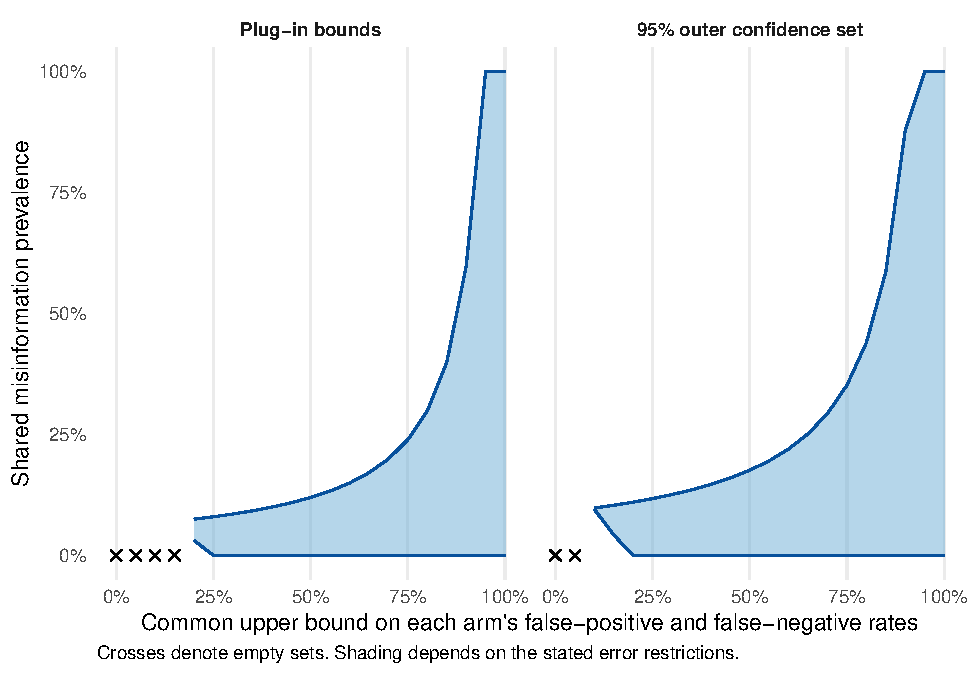
\includegraphics[width=\linewidth]{identification_sensitivity.pdf}
\caption{Prevalence depends on restrictions on both error directions}
\label{fig:sensitivity}
\begin{minipage}{\linewidth}
\footnotesize\emph{Note:} Both arms share the horizontal-axis cap on false positives and false negatives. Shaded intervals intersect the arm-specific bounds. The left panel uses observed rates; the right propagates simultaneous binomial uncertainty. Crosses mark empty sets at evaluated grid points. The 5-percentage-point grid is joined for display; exact calculations are provided in the replication files.
\end{minipage}
\end{figure}

\section{Implications for measurement and study design}

A useful measure must specify both its target and its possible mistakes. If the target is stored misinformation, researchers should state the proposition and truth key, the time at which belief is defined, the conceptual confidence threshold, the respondent population, and the response event used as evidence. A rate of confidently incorrect responses can be reported directly. Calling it the prevalence of misinformation adds a claim about the channel.

The most tenable starting point allows both false positives and false negatives. Questions can induce answers, and respondents can withhold or understate beliefs. Neither direction needs to dominate everywhere. An informative partial-identification analysis then needs substantive evidence for limits on these errors. When no such evidence exists, an uninformative bound is an accurate description of what has been learned about the stored state, alongside potentially informative findings about responses.

Validation effort should target the assumptions that matter for the estimand. Identifying only misinformation may require less calibration than recovering all five states. Cognitive interviews, records of prior statements, repeated measurements, and controlled validation tasks can probe different parts of the channel. None automatically supplies error-free ground truth: prior statements may themselves be expressive, repeated questions may change beliefs, and controlled tasks may not transport. Their value is in supporting or challenging specific restrictions rather than certifying an instrument in the abstract.

Format randomization has a useful but limited role. It identifies how elicitation changes response distributions and can test the compatibility of proposed measurement restrictions across formats. It does not explain the response changes by itself. Incentives or additional prompts likewise identify effects on answers under their designs; interpreting those effects as removal of partisan expression or guessing requires further assumptions about other response pathways and the underlying belief state.

Our earlier empirical comparisons and reconstructed historical models remain reproducible in the accompanying repository. They describe format effects, scoring sensitivity, correlates, and response profiles. Those findings cannot by themselves establish the size of an ignorant public, identify a guessing mechanism, or validate cognitive labels for latent response classes. They are separate from the formal contribution developed here.

The Casablanca distinction survives this caution. Rick's false belief and Rick's absence of belief remain substantively different. A questionnaire can help distinguish them, but only through a defensible account of how each state would produce an answer. The appropriate claim is the one supported by that account: an observed response distribution, a range of possible belief prevalences, or, where the channel is sufficiently known, an identified prevalence.

\clearpage
\bibliographystyle{apsr}
\bibliography{references}

\clearpage
\appendix
\section{Proofs and scope of the results}
\label{app:proofs}

\subsection{Known-channel identification}

If $A$ has full column rank, $A\pi=q$ has at most one solution. Conversely, rank deficiency supplies a nonzero $d$ with $Ad=0$. Because each block of $A$ is column stochastic, $\mathbf1'$ belongs to its row space, so $\mathbf1'd=0$. At an interior composition, sufficiently small positive and negative perturbations $\pi\pm\epsilon d$ remain in the simplex and generate the same $q$. Hence the full composition is not globally identified.

If $c$ lies in the row space, write $c'=b'A$. Then $c'\pi=b'q$ is observed. If it does not, there is a null vector $d$ with $c'd\ne0$. The same interior perturbations yield distinct values of the functional at the same $q$. This proves Proposition~\ref{prop:rank}, including its interior qualification. Nonnegativity may eliminate those perturbations at boundary compositions, which is why the qualification matters.

\subsection{Binary sharpness and intersections}

At a fixed $p$, the attainable response probabilities are exactly
\[
 [(1-\beta)p,\;\alpha+(1-\alpha)p].
\]
The endpoints set $(f,s)$ to $(0,1-\beta)$ and $(\alpha,1)$, respectively. The image of the rectangular admissible set under the linear map $f(1-p)+sp$ is the entire interval. Inverting its two inequalities gives \eqref{eq:bounds}, with the stated conventions when a denominator vanishes.

Explicitly, for a feasible $p$, let
\[
 D=\alpha(1-p)+\beta p,\qquad
 t=\frac{q-(1-\beta)p}{D}.
\]
If $D>0$, feasibility implies $t\in[0,1]$; choose $f=t\alpha$ and $s=1-\beta+t\beta$. These parameters reproduce $q$. If $D=0$, the attainable interval is a singleton and its endpoint construction suffices. This proves sharpness for one arm.

For every $p$ in the intersection, construct an admissible $(f_z,s_z)$ separately for each arm. A joint distribution of potential responses exists, for example by drawing them independently conditional on the premeasurement state using these kernels. This is a construction proving existence, not an empirical assumption of conditional independence. With no additional cross-format restrictions, every point of the intersection is attainable. Constraints such as common channels or monotone individual potential responses would define a different model and may narrow its set.

\subsection{The finite-state linear program}

Any admissible $(A_z,\pi)$ generates joint masses satisfying \eqref{eq:lp}. Conversely, take a feasible solution. For $\pi_s>0$, set $A_z(r,s)=x_{zrs}/\pi_s$. The column sums and entrywise bounds follow directly. For $\pi_s=0$, choose any stochastic column within its bounds; \eqref{eq:validcolumns} guarantees that one exists. Every feasible solution therefore corresponds to an admissible response model, proving sharpness. The same program accepts intervals on response probabilities by replacing each response-margin equality with lower and upper inequalities. These intervals must jointly admit probability distributions.

\section{Sampling uncertainty and reproducibility}
\label{app:inference}

For an arm with $n_z$ assigned respondents, $a_z$ observed positives, and $m_z$ missing answers, the sample response probability is bounded by $[a_z/n_z,(a_z+m_z)/n_z]$ without assuming anything about missing answers. Proposition~\ref{prop:bounds} uses the lower endpoint for its lower bound and the upper endpoint for its upper bound. This treats the missing respondents as potentially positive or negative while retaining the assigned-arm population.

For the illustration's two fully observed arms, we construct a 97.5\% two-sided Clopper--Pearson interval for each binomial probability. Bonferroni's inequality gives at least 95\% simultaneous coverage. Propagating the lower and upper probability limits through the bound functions and intersecting across arms gives an outer confidence set for the population identified set under the maintained error restrictions. The calculation is conservative and conditional on independent within-arm sampling from the respondent population. It is not a design-exact finite-population randomization interval and does not address selection into this convenience sample.

The code also handles missing responses. In that case it uses one lower confidence limit for the observable positive event and one upper confidence limit for the event ``positive or missing'' in each arm, allocating the familywise error probability equally across these four one-sided limits. Their lower and upper limits bound the corresponding partially observed response probabilities without a missing-at-random assumption. Channel uncertainty and sampling uncertainty remain distinct: the caps specify the former, the binomial intervals the latter. None of these calculations covers a wrongly keyed proposition.

The replication package is available at \href{https://github.com/finite-sample/know_casablanca}{\nolinkurl{github.com/finite-sample/know_casablanca}}. Stage 09 generates every empirical number, table, and figure in this manuscript from the checked survey files. It also implements the multicategory linear program and tests it against analytic cases, observational-equivalence examples, and boundary and incompatibility cases. Stages 01--08 retain the earlier descriptive and historical analyses. The design note documents the illustration's retrospective status, item choice, and assumptions; separate reports distinguish those other analyses from this manuscript's identification claims.

\end{document}
